\section{Anexos}

Se puede observar en el artículo correspondiente a un trabajo similar sobre las comorbilidades del SARS-Cov2 (\cite{Sanyaolu2020}) se han decidido incluir las dos primeras gráficas que ofrecen datos interesantes respecto a diferentes fenotipos que se han ido recogiendo desde la aparición y adquisición de mayor relevancia de la enfermedad (desde enero de 2020 hasta marzo del mismo año) así como una comparativa de las diferentes condiciones patológicas preexistentes que favorecen la aparición y afección.

\begin{figure}[h!]
		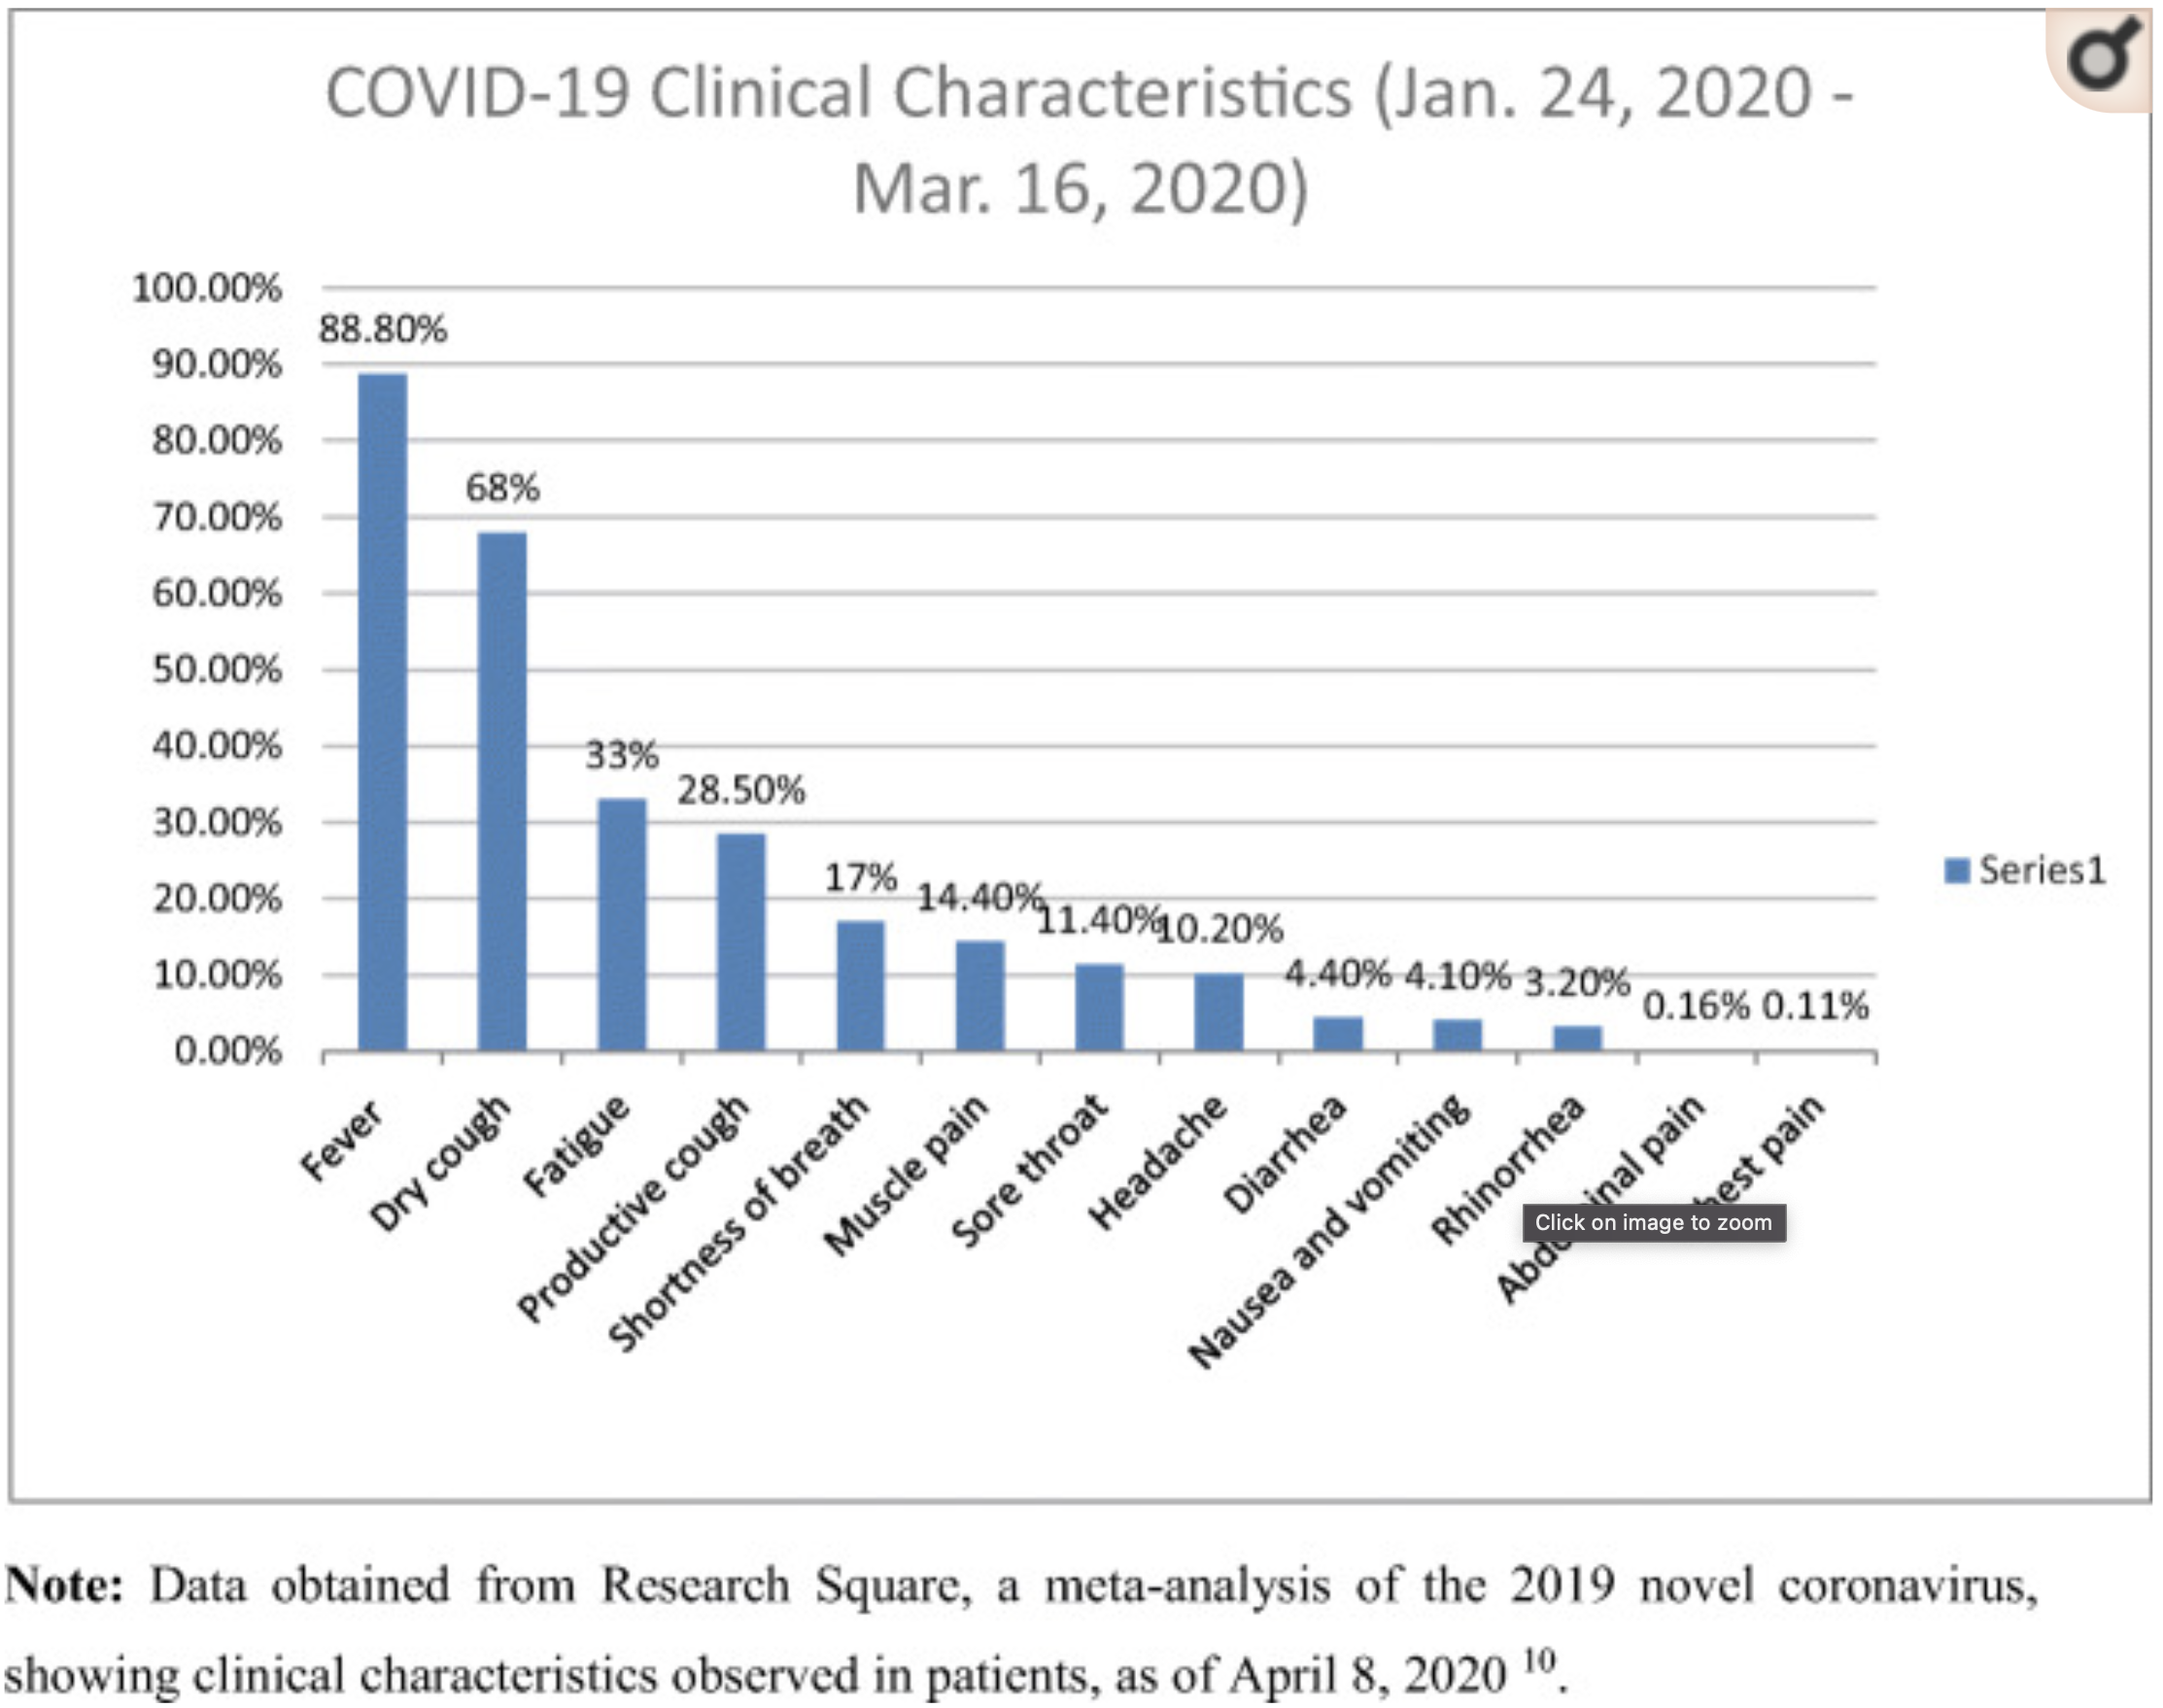
\includegraphics[width=0.9\textwidth]{figures/COVIDClinCharac.png}
		\caption{SARS-CoV-2 Clinical Characteristics}
		\label{fig:covid_clin_char}
	\end{figure}
	
	\begin{figure}[h!]
		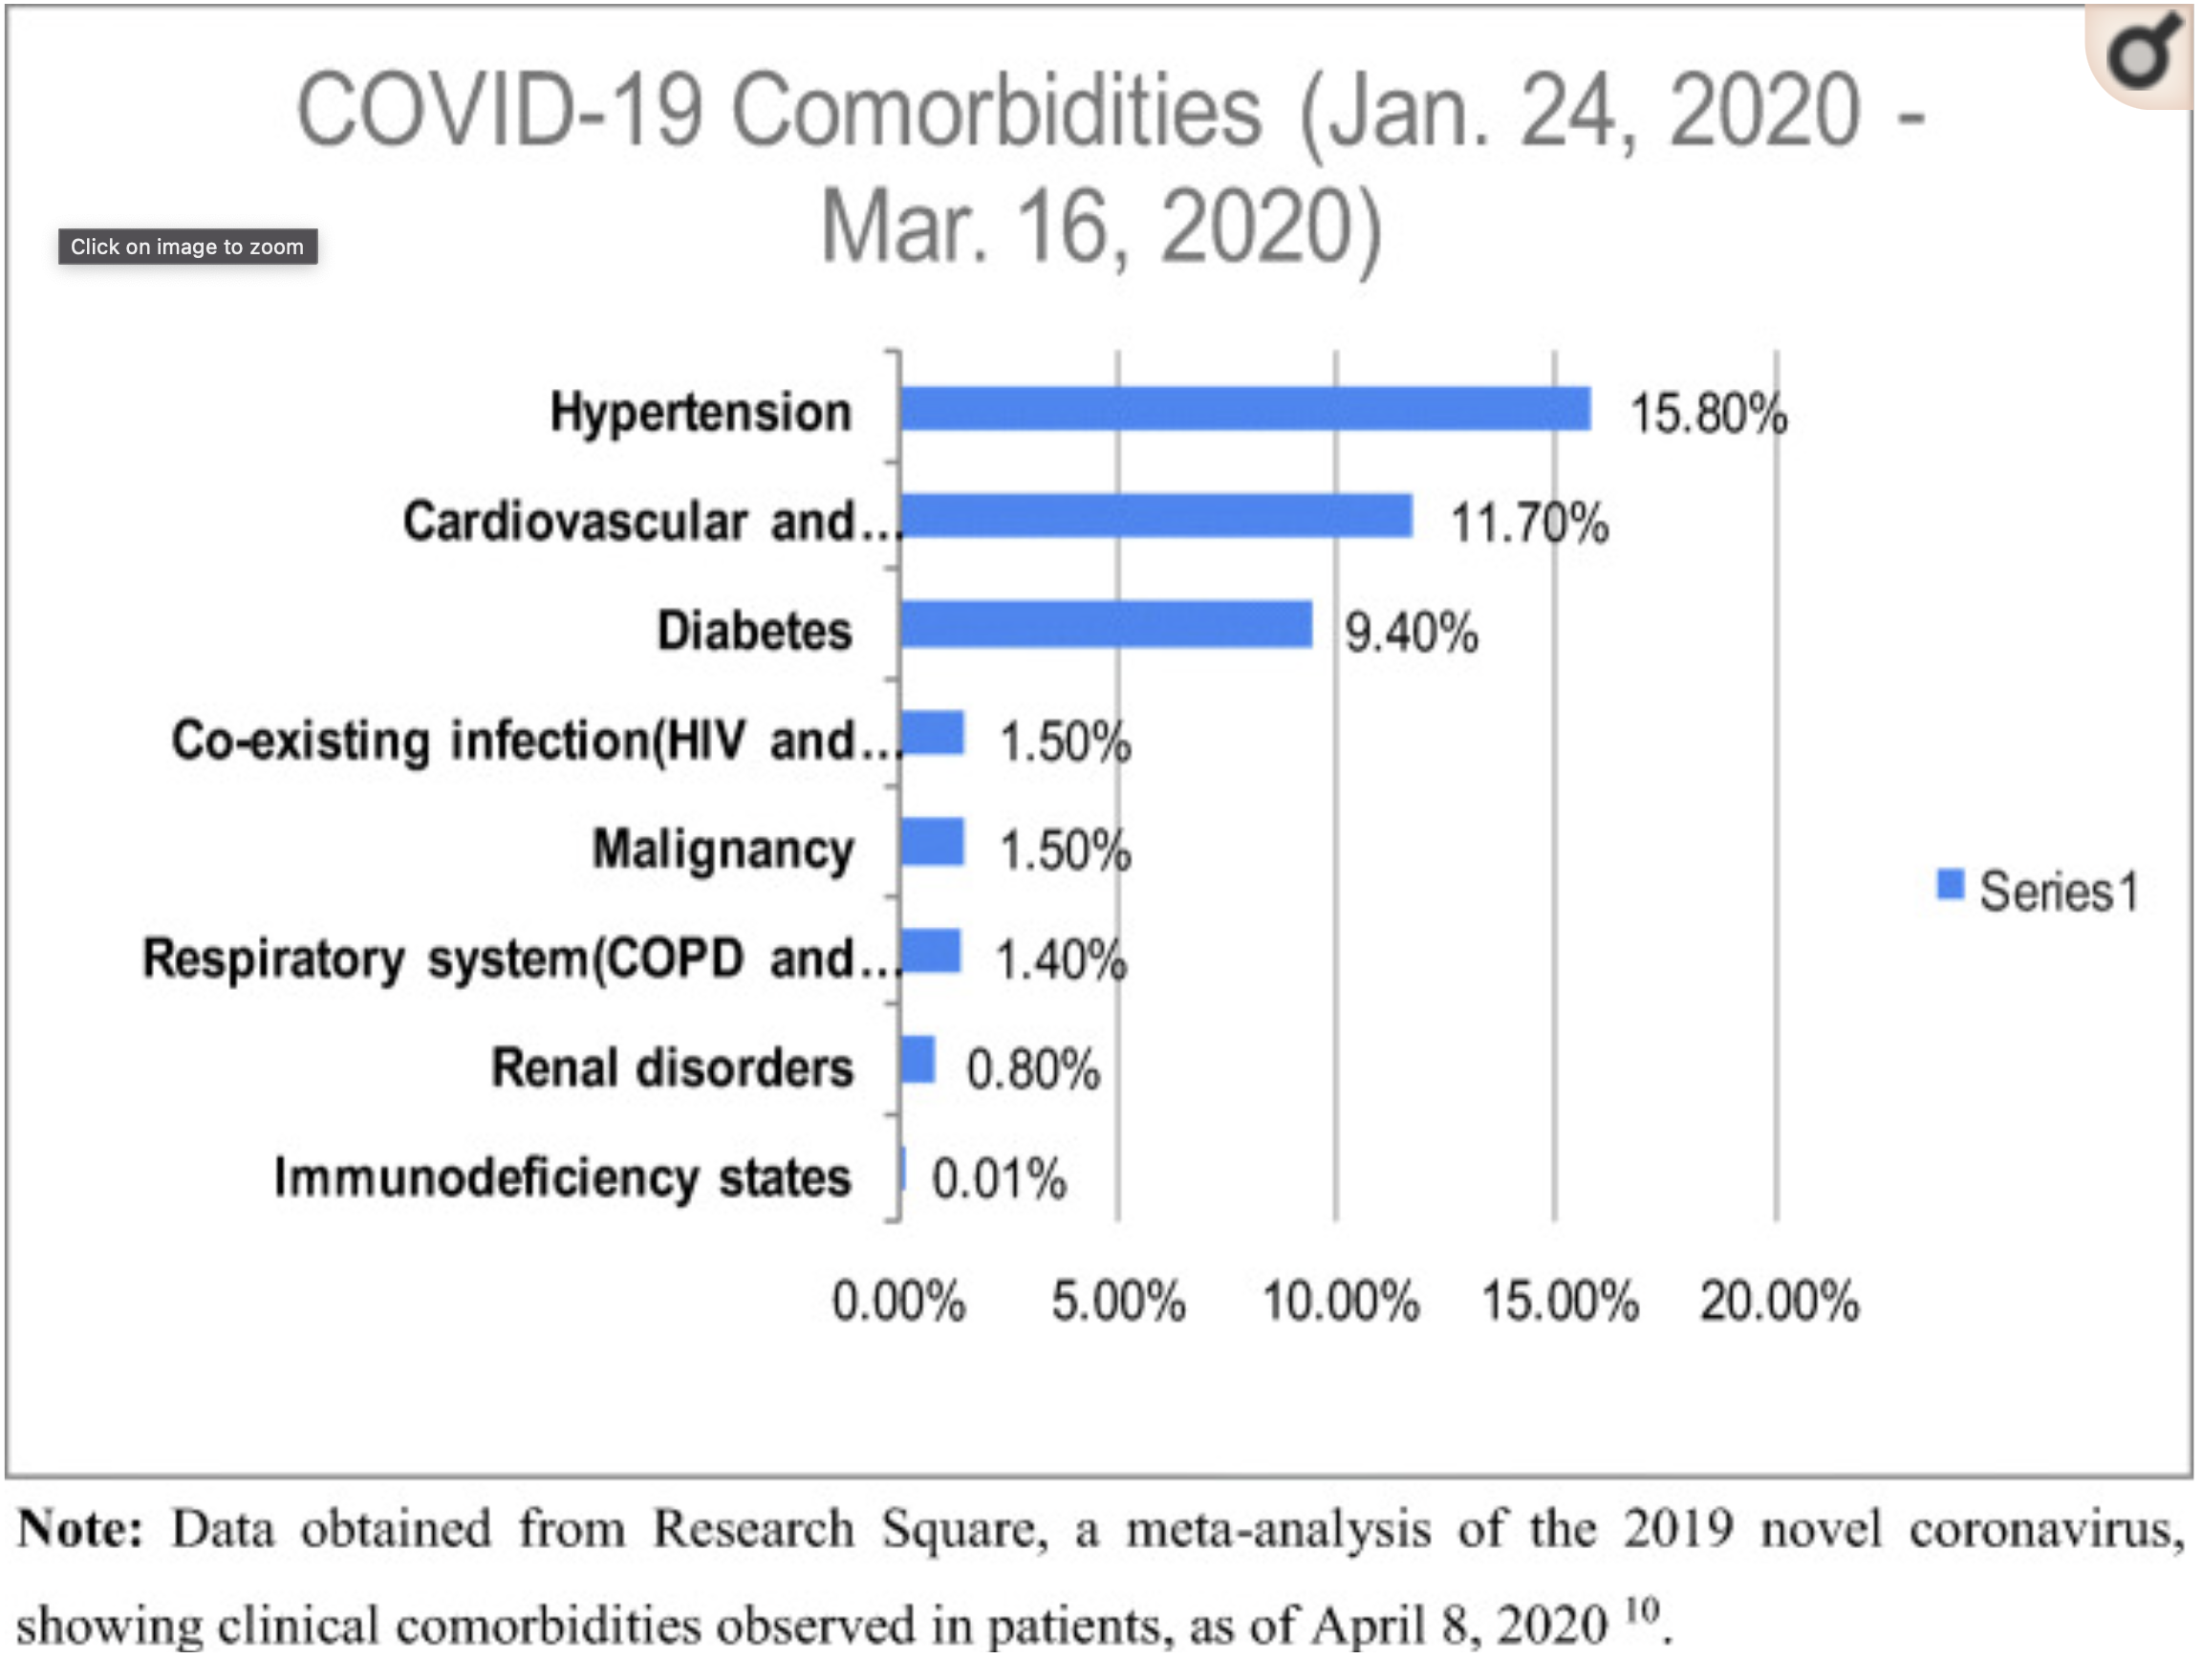
\includegraphics[width=0.9\textwidth]{figures/COVIDComorb.png}
		\caption{SARS-Cov2 Comorbities}
		\label{fig:covid_comorb}
	\end{figure}
